\documentclass[a4paper,12pt]{article}
\usepackage[frenchb]{babel}
\usepackage[utf8]{inputenc}
\usepackage[T1]{fontenc} 
%Pour avoir un rendu plus beau
\usepackage{lmodern}
\usepackage{float}
\usepackage{graphicx}
\usepackage{geometry}
\usepackage{amsmath}
\usepackage{array}
\usepackage{tikz}
\usepackage{hyperref}
\usepackage{pdfpages}
\usepackage{bigfoot}
\usetikzlibrary{trees}

\geometry{margin=2cm}

\begin{document}
\begin{center}
  
\includegraphics [width=40mm]{ENSEIRB-MATMECA.jpg}

\vspace{\stretch{1}}

\textsc{\Huge Flots et Combinatoire :}\\
\vspace{0.5cm}
\textsc{\Huge Optimisation d'un réseau de communication}\\
\rule{0.4\textwidth}{1pt}

\vspace{\stretch{1}}

\begin{center}
  
  \begin{flushleft}
    {\large
    \emph{Auteur :}}\\
    Ludovic Hofer
  \end{flushleft}
  
  
  \begin{flushright}
    {\large
    \emph{Responsables :}}\\
    \begin{tabular}{l r}
      Responsable de l'UE : & François Vanderbeck\\
      Chargé de TD : & Pierre Pesneau
    \end{tabular}
  \end{flushright}
\end{center}

\vspace{\stretch{1}}

{\large \url{https://github.com/medrimonia/reseauTelecom/}}

\vspace{\stretch{1}}
                  
{\large Deuxième année, filière informatique}

~

{\large Second Semestre}\\
                  
\end{center}
\thispagestyle{empty}
\pagebreak

\tableofcontents
\pagebreak

\section{Introduction}
Le travail présenté dans ce document s'inscrit dans le cadre du cours de
flots et combinatoire. Ce projet permet aux étudiants d'appréhender des
méthodes d'approximation de problèmes \verb!NP-Complets!.\\

\subsection{Description du problème}
Le problème a résoudre se présente sous la forme suivante :\\
Plusieurs sommets doivent être reliés afin de former un réseau, le coût d'une
arête est donné par la distance entre les deux sommets qu'elle relie. Il faut
que le graphe obtenu après ajout des arêtes soit connexe afin de permettre
à chaque routeur d'envoyer des messages à tous les autres. Mais cette
condition n'est pas suffisante, effectivement, pour assurer la stabilité du
réseau, il est demandé que pour tout couple de sommets, il existe au moins
deux chemins différents n'ayant aucune arête en commun. De plus, afin
d'éviter que toutes les communications empruntent le même chemin, il est
exigé que toutes les arêtes soient dans un cycle de longueur $k$ au
maximum\footnote{Ce $k$ étant variable, il est nécessaire que le programme
puisse s'adapter à un changement de celui-ci, même si son ordre de grandeur
était fixé aux environs de 4.}.

\subsection{Formalisation du problème}
Ce problème peut être décrit comme un problème de recouvrement des sommets par
l'ensemble des cycles. En cherchant à minimiser la somme du poids des arêtes
présentes dans un cycle ou plus. Une contrainte supplémentaire à celle du
problème de recouvrement est qu'il faut assurer la connexité du graphe obtenu.

\section{Développement}

Même si la majorité du développement a été faite en \verb!c++!, j'ai aussi
utilisé d'autres langages, par exemple le \verb!python! pour générer du code
tikz permettant de visualiser les graphes en les intégrant dans des documents
latex.

\subsection{Visualisation des graphes}
Afin de pouvoir facilement détecter des problèmes dans les résultats fourni
par le programme, j'ai commencé par développer un petit module en python
permettant de transformer un graphe au format texte en graphe visualisable
par \verb!tikz!.
J'ai choisi d'utiliser le langage \verb!python! car il permet de parser très
facilement du texte et il convient donc parfaitement aux genres d'objectifs
de cette partie du programme.

\begin{figure}
  \resizebox{\columnwidth}{!}{
\begin{tikzpicture}
\tikzstyle{every node}=[font=\huge]
\draw [fill=violet] ( 8.8 , 5.050000000000001 ) rectangle ( 9.0 , 5.25 );
\node at ( 8.9 , 5.95) { 003 };
\draw [fill=violet] ( 11.15 , 12.15 ) rectangle ( 11.35 , 12.35 );
\node at ( 11.25 , 13.05) { 002 };
\draw [fill=violet] ( 1.9500000000000002 , 5.300000000000001 ) rectangle ( 2.1500000000000004 , 5.5 );
\node at ( 2.0500000000000003 , 6.2) { 001 };
\draw [fill=violet] ( 1.25 , 12.000000000000002 ) rectangle ( 1.4500000000000002 , 12.200000000000001 );
\node at ( 1.35 , 12.900000000000002) { 000 };
\draw [fill=violet] ( 8.05 , 8.950000000000001 ) rectangle ( 8.25 , 9.15 );
\node at ( 8.15 , 9.850000000000001) { 007 };
\draw [fill=violet] ( 1.55 , 3.8000000000000003 ) rectangle ( 1.7500000000000002 , 4.0 );
\node at ( 1.6500000000000001 , 4.7) { 006 };
\draw [fill=violet] ( 11.450000000000001 , 2.5500000000000003 ) rectangle ( 11.65 , 2.7500000000000004 );
\node at ( 11.55 , 3.45) { 005 };
\draw [fill=violet] ( 4.250000000000001 , 10.3 ) rectangle ( 4.45 , 10.5 );
\node at ( 4.3500000000000005 , 11.200000000000001) { 004 };
\draw [fill=violet] ( 12.3 , 5.4 ) rectangle ( 12.5 , 5.6 );
\node at ( 12.4 , 6.3) { 009 };
\draw [fill=violet] ( 6.050000000000001 , 9.9 ) rectangle ( 6.25 , 10.1 );
\node at ( 6.15 , 10.8) { 008 };
\draw [ultra thick, violet] ( 1.35 , 12.100000000000001 ) -- ( 4.3500000000000005 , 10.4 );
\draw [ultra thick, violet] ( 1.35 , 12.100000000000001 ) -- ( 6.15 , 10.0 );
\draw [ultra thick, violet] ( 2.0500000000000003 , 5.4 ) -- ( 4.3500000000000005 , 10.4 );
\draw [ultra thick, violet] ( 2.0500000000000003 , 5.4 ) -- ( 1.6500000000000001 , 3.9000000000000004 );
\draw [ultra thick, violet] ( 11.25 , 12.25 ) -- ( 8.15 , 9.05 );
\draw [ultra thick, violet] ( 11.25 , 12.25 ) -- ( 12.4 , 5.5 );
\draw [ultra thick, violet] ( 8.9 , 5.15 ) -- ( 11.55 , 2.6500000000000004 );
\draw [ultra thick, violet] ( 8.9 , 5.15 ) -- ( 8.15 , 9.05 );
\draw [ultra thick, violet] ( 8.9 , 5.15 ) -- ( 12.4 , 5.5 );
\draw [ultra thick, violet] ( 4.3500000000000005 , 10.4 ) -- ( 1.6500000000000001 , 3.9000000000000004 );
\draw [ultra thick, violet] ( 4.3500000000000005 , 10.4 ) -- ( 8.15 , 9.05 );
\draw [ultra thick, violet] ( 11.55 , 2.6500000000000004 ) -- ( 12.4 , 5.5 );
\draw [ultra thick, violet] ( 8.15 , 9.05 ) -- ( 6.15 , 10.0 );
\end{tikzpicture}
}
Total cost : 1088.75

Time used : 15.3759 ms

\end{figure}

\subsection{Architecture}
L'ordre de traitement utilisé pour obtenir une solution approximant
le problème est le suivant :

\begin{itemize}
\item Acquisition du graphe : Lire un graphe depuis un fichier.
\item Création de l'arbre couvrant minimal
\item Complétion du graphe afin de satisfaire toutes les contraintes.
\item Filtre
\item Sauvegarde du résultat dans un fichier
\end{itemize}

Au coeur du programme \verb!c++! se trouve la classe \verb!Graph! qui permet de
nombreuses opérations sur les graphes. Au vu de la nature spécifique du
problème, \footnote{Graphe complet non orienté sans boucles dont le poids des
arêtes correspond à la distance entre la position des sommets.} j'ai pensé
qu'il n'était pas nécessaire de faire une classe pour les arêtes. Lors du
développement, j'ai pu constaté qu'un bon nombre de tâches auraient pu être
simplifiées si j'avais fait ce choix dès le début.
\\
Cette classe stocke donc les sommets dans un vecteur, la présence des arêtes
dans une matrice d'incidence de booléens, et le poids des arêtes dans une
matrice de floats\footnote{Cette donnée n'est à priori pas nécessaire puisque
les coordonnées des sommets restent disponibles, cependant, il est plus efficace
de ne calculer qu'une seule fois la racine carrée nécessaire à l'obtention de la
distance}.
\\
Outre sa capacité de stockage, cette classe permet aussi à l'utilisateur
d'utiliser des méthodes permettant par exemple de générer des cycles de longueur
inférieure ou égale à $k$, contenant deux sommets tout en spécifiant la méthode
de calcul des scores des différents cycles. Bien évidemment, il existe aussi une
méthode permettant de vérifier si le graphe respecte les contraintes du
problème. Le but initial de cette approche était de permettre d'expérimenter
rapidement différentes approches de résolution du problème simplement en
utilisant plusieurs méthodes successivement afin d'approcher le résultat. En
pratique, je me suis finalement limité à deux versions qui seront comparées dans
la partie résultats.

\subsection{Algorithmes utilisés}
Même s'il n'existe pas actuellement d'algorithmes résolvant le problème qui nous
a été donné dans un temps polynomial, il existe une multitude d'algorithmes
connus qui peuvent servir dans la recherche d'une approximation de la solution.
Afin de ne pas réinventer la roue, je me suis donc servi de méthodes éprouvées
pour certains sous-problèmes.

\subsubsection{Recherche de l'arbre couvrant minimal}
Le calcul de l'arbre couvrant minimal permet de satisfaire la contrainte
de connexité du graphe. Il permet d'obtenir une bonne base à partir de laquelle
rechercher des solutions qui respectent toutes les contraintes du problème.
Afin de calculer l'arbre couvrant minimal, je me suis donc servi de l'algorithme
de {\em Prim}.

\subsubsection{Ajout d'arêtes afin de satisfaires les contraintes}
À partir de l'arbre couvrant minimal, on peut satisfaire la contrainte que
toutes les arêtes soient dans des cycles de longueur $k$ ou moins en se
contentant d'ajouter des arêtes. Pour cette étape, j'ai conservé deux solutions
différentes :
\begin{itemize}
\item {\em Ajout d'arêtes en observant individuellement chaque arête :}\\
  Le principe de cette méthode était uniquement de mettre toutes les arêtes de
  l'arbre couvrant minimal dans une file et de vider cette file en vérifiant
  pour chaque arête si elle était présente dans un cycle ou non. Dans le cas où
  la contrainte n'était pas respectée, on la comblait en ajoutant l'ensemble
  d'arêtes de poids total minimum permettant de respecter cette contrainte
  \footnote{Ce problème s'apparentant à la recherche du plus court chemin dans
    un graphe ou les arêtes déjà présentes ont un poids de zéro et où l'arête
    examinée a un poids infini.}.
\item {\em Recouvrement de l'arbre minimal par un ensemble de cycle :}\\
  Le principe de cette approche est de recouvrir l'ensemble des arêtes de
  l'arbre couvrant minimal par des cycles de longueur $k$ ou inférieure. Si l'on
  pouvait choisir l'ensemble de cycles de poids minimal satisfaisant cette
  contrainte, l'on serait extrêmement proche de la solution idéale du problème,
  mais comme le {\em set covering problem} est \verb!NP-dur!, il est nécessaire
  d'approximer sa solution, l'approche que j'ai choisie étant de générer un
  nombre limité de cycles et, tant que l'ensemble n'est pas recouvert, d'ajouter
  le cycle obtenant le meilleur score.
  \footnote{Les deux principales méthode d'obtention des scores étant dans un
    cas le poids ajouté et dans l'autre cas le poids ajouté divisé par le nombre
    d'arêtes de l'arbre couvrant minimal recouvertes}
\end{itemize}

\subsubsection{Filtres}
Pour tout graphe donné, il peut exister des améliorations assez simples
qui permettent de réduire le poids total des arêtes sans violer de contraintes.
Dans certains exemples obtenus, certaines arêtes pouvaient par exemple être
purement et simplement enlevées sans qu'aucune des contraintes ne soit violée.
J'ai donc fourni deux filtres permettant de diminuer le coût total une fois la
génération finie.
\begin{itemize}
\item Suppression d'une arête :
  Ce filtre consiste uniquement à essayer d'enlever les arêtes l'une après
  l'autre en vérifiant que les contraintes sont respectées. Le problème de
  cette technique est qu'elle ne per
\item Modification d'une arête :
  Ce filtre consiste à prendre une arête et à essayer de remplacer une de ses
  extrêmités par un autre sommet, plus proche du sommet conservé. Si cette
  modification n'engendre pas une violation de contrainte, l'arête est
  remplacée. Dans le cas où plusieurs arêtes répondent à cette condition, celle
  dont le poids est minimal est conservée. Ce processus peut être itéré
  plusieurs fois car une amélioration peut en permettre une qui était impossible
  auparavant.
\end{itemize}

Si ces filtres ne permettent pas d'obtenir la meilleure solution, ils
fournissent en tout cas la garantie de ne pouvoir qu'améliorer la solution étant
donné que toute modification qu'ils apportent est forcément positive. En
revanche, l'ordre idéal d'application de ces filtres n'est pas évident et peut
varier suivant les instances.

\section{Résultats}

Les deux exécutables différents dont je me suis servi se basent sur la démarche
décrite dans la section {\em Architecture}. La différence se situe au niveau de
la manière dont est complété l'arbre couvrant minimal afin de respecter les
contraintes d'appartenance aux cycles pour les arêtes.\footnote{Les deux
  techniques étant décrites précédemment}

\begin{itemize}
\item {\textbf cycle} : Utilisation de l'ajout simple d'arête.
\item {\textbf cycleV2} : Utilisation du recouvrement de l'arbre couvrant par
  des cycles.
\end{itemize}

Tous les graphiques présents dans cette section reflètent les résultats obtenus
pour des exécutions sur l'ensemble des fichiers de données qui nous ont été
fournis avec une valeur de $k$ fixée à 4. Bien qu'il soit possible d'exécuter
le programme avec d'autres valeurs de $k$.

\subsection{Qualité des solutions}
N'ayant pas les solutions optimales du jeu de données fourni, il n'est pas
possible de déterminer à quel distance la solution fournie par le programme est
de la solution optimale. Cependant, il est possible d'avoir deux observations
d'ordre générale au point de vu des résultats obtenus :
\begin{itemize}
\item Les résultats obtenus sont généralement bien meilleurs que ceux que l'on
  aurait obtenu en essayant de trouver une solution sans l'aide d'un ordinateur.
  Sur une notion évolutive, les résultats se sont amélioré de façon
  significative par rapport aux premières versions du programme.
\item Il reste des graphes obtenus ou l'affichage permet à un humain de déceler
  facilement certaines imperfections \footnote{Croisement d'arêtes sur le plan
    par exemple.}.
\end{itemize}
Il est donc flagrant que le programme présenté ici ne présente pas les meilleurs
résultats que l'on peut obtenir sur ce problème à l'aide d'un ordinateur.

\begin{figure}[H]
  \caption{Comparaison des deux méthodes}
  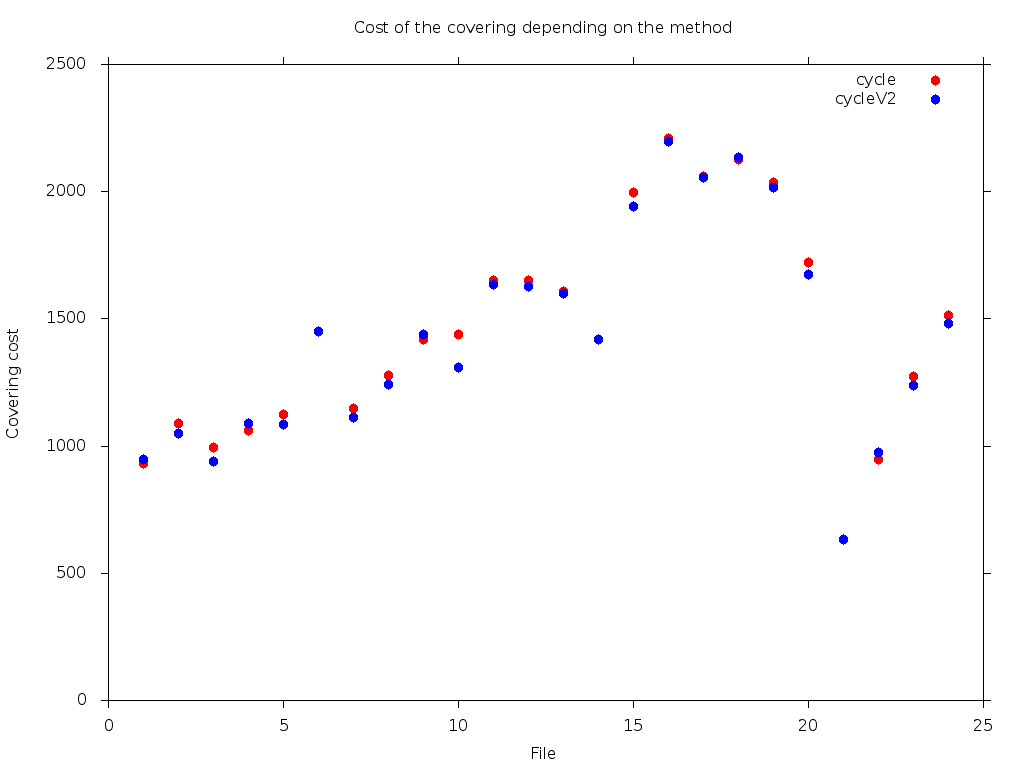
\includegraphics[width = \textwidth]{comparison.png}
\end{figure}

On peut voir sur ce graphique que la différence de qualité des solutions n'est
pas si grande et que bien que la solution obtenue par la méthode utilisant la
couverture de l'arbre minimal soit généralement meilleure, ce n'est pas toujours
le cas. Il parait donc adéquat d'utiliser les deux méthodes et de retenir
le meilleur résultat obtenu lorsque c'est possible.

\subsection{Temps d'exécution}
L'aspect primordial de cette résolution de problème est d'éviter de tomber dans
une complexité exponentielle par rapport au nombre de sommets. J'ai pu évité ce
problème là, en revanche, certaines fonctions utilisées ont un complexité
exponentielle par rapport à $k$, mais comme ce nombre n'est pas sensé grandir
proportionnellement au nombre de sommets et qu'il a été exprimé qu'il resterait
de toute façon très petit, ce problème n'est pas si gênant.
\\
Un calcul complet de la complexité n'a pas été effectué et il m'est évident
qu'il reste de nombreuses optimisations possibles dans le code présenté.
Cependant une première approximation de la différence de complexité et du temps
d'exécution des deux méthodes peut être observé grâce à l'expérience

\begin{figure}[H]
  \caption{Comparaison du temps d'exécution des deux méthodes}
  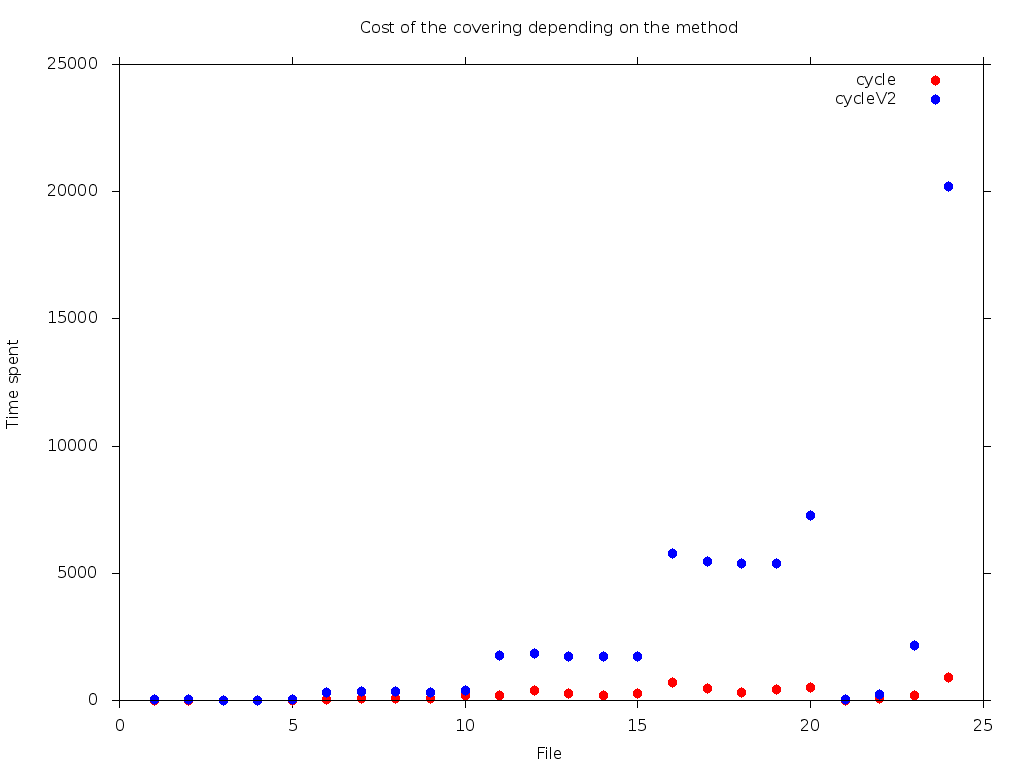
\includegraphics[width = \textwidth]{time_comparison.png}
\end{figure}

Il est important pour la compréhension de ce graphique de souligner le fait que
les fichiers de données fournis comportent un nombre de sommets compris dans
l'ensemble $\{10,20,30,40\}$ pour les 20 premiers fichiers (5 de chaque). Les
quatres dernier fichiers comportant respectivement $12,17,29,52$ sommets.
\\
Ce graphe laisse donc à penser que la seconde solution a une complexité
asymptotique plus élevée que la première. La majorité du temps utilisé dans la
seconde est en fait dû à la génération des cycles, bien que ceux-ci soit peu
nombreux à être généré, leur création reste assez gourmande. Il semble donc
clair que dans ce cas, pour un grand nombre de sommets, on aura tendance à
préférer la première version. Tandis que si le temps n'est pas une contrainte
bloquante pour la seconde version, l'utilisation combinée des deux fournira les
meilleurs résultats.


\section{Perspectives}
Dans le cadre de ce projet, il y a certains aspects qui m'intéressaient mais qui
n'ont pas pu être exploité par manque de temps.

\subsection{Utilisation de l'aléatoire}
Le cours d'algorithmique probabiliste que j'ai suivi lors du dernier semestre
m'a sensibilisé aux problèmes de mauvaises instances qui me semblent très
présent dans le programme que j'ai créé, en effet, certains filtres ou autre
traitements se basent sur l'ordre dans lequel sont disposés des éléments au sein
d'une liste et un ordre différent pourrait résulté sur des performances bien
meilleur. Je serai donc particulièrement intéressé à voir la manière dont
s'améliorent les solutions en répétant plusieurs fois certaines étapes/filtres
une fois la composante aléatoire installée.

\subsection{Fichier de configuration}
Au vu du développement que j'ai effectué, j'aurais aimé pouvoir approfondir un
peu certains aspects de configuration, permettant ainsi de définir de nouvelles
approches ou de changer l'ordre d'opérations sans avoir à recompiler quoique ce
soit et en ayant un seul exécutable. J'imaginais par exemple utiliser des
fichiers xml pour décrire la procédure à suivre. Dans l'idéal le but était de
fournir au programme un fichier de configuration de cette forme-ci:
\begin{verbatim}
<program>
    <generationMethod name="Covering"/>
    <filters>
        <filter name="edgeRemoval" randomized="true" nbRuns="10"/>
        <filter name="edgeSwitch" randomized="false" nbRuns="1"/>
    </filters>
</program>
\end{verbatim}
Si l'idée est relativement simple, son implémentation m'aurait demandé un temps
que je n'avais malheureusement pas.

\section{Conclusion}
Il a été très intéressant de pouvoir travailler sur des méthodes permettant
d'approximer la solution à un problème \verb!NP-complet! en se basant sur des
algorithmes déjà existant. La comparaison des différentes méthodes a aussi été
intéressantes. Je pense qu'il faudrait de nouveaux filtres pour améliorer la
qualité des solutions trouvées.
\\
Le principal problème dans ce projet a été le manque de temps, en effet, avec
les nombreux projets que l'on réalise, il est difficile de consacrer autant de
temps qu'on le souhaite à chacun des projets. Cependant je suis content d'avoir
pu effectuer ce projet seul, mon expérience des projets de groupe dans le cadre
de l'ENSEIRB-MATMECA n'étant pas des plus transcendante.

\end{document}
